\chapter{La Revolución No Contrastiva: Decorrelación y el Principio de Barlow}
\label{cap:nocontrastive}

La búsqueda de métodos independientes de las muestras negativas condujo a una de las intersecciones más ricas entre la neurobiología teórica y el aprendizaje de representaciones: la aplicación del principio de Barlow. Este capítulo detalla los fundamentos matemáticos de las pérdidas basadas en la correlación cruzada (Barlow Twins) y la regularización explícita de covarianza (VICReg).

\section{La Hipótesis de Reducción de Redundancia de Barlow (1961)}
\label{sec:barlow_hipotesis}
En 1961, el neurobiólogo Horace Barlow formuló la \textbf{hipótesis de codificación eficiente}, planteando que nuestro sistema nervioso no procesa los estímulos sensoriales en bruto, sino que los recodifica de modo que la actividad de las neuronas individuales sea, en la medida de lo posible, estadísticamente \textit{independiente} \cite{barlow1961possible}. La idea se apoyaba en trabajos previos de Shannon, quien había mostrado que sistemas naturales como el lenguaje contienen una redundancia considerable. En ellos, gran parte de la señal es predecible a partir del resto, y por tanto no aporta información nueva en el sentido de Shannon. Una codificación óptima, bajo esta perspectiva, es aquella que elimina dicha redundancia y representa la señal con el menor número de símbolos estadísticamente correlacionados entre sí.

Al trasladar este principio a la biología, Barlow observó que nuestro entorno presenta fuertes correlaciones espaciotemporales. Por ejemplo, la luminancia en regiones contiguas del campo visual rara vez varía de forma abrupta, de manera que transmitir cada píxel o cada instante de forma independiente supondría malgastar buena parte de la capacidad del canal neuronal en información redundante, con un coste metabólico que el cerebro no puede permitirse. Para resolverlo, la corteza sensorial actuaría como un filtro que suprime esa redundancia, proyectando las señales de entrada sobre un nuevo espacio de características mutuamente independientes. La red, así, no necesita gastar recursos en lo que ya es predecible a partir del contexto inmediato, y puede reservarlos para aquello que realmente constituye información nueva.

\subsection{La Información Mutua como Medida Ideal de Independencia}

Para formalizar la hipótesis de reducción de redundancia de Barlow, el objetivo es asegurar que las componentes del vector de \textit{embeddings} $Z = (z_1, z_2, \dots, z_d)$ extraído por un modelo sean lo más independientes posible.

En estadística elemental, la independencia suele aproximarse mediante la \textbf{correlación lineal} de Pearson ($\rho$). Sin embargo, como principal limitación, ésta solo detecta relaciones lineales. Para medir la dependencia de forma exhaustiva y fiel, la métrica ideal es la \textbf{Información Mutua} ($I$) de la teoría de la información de Shannon \cite{shannon1948mathematical}. A diferencia de la correlación, la información mutua captura \textit{cualquier} tipo de dependencia (lineal o no lineal) y es invariante ante transformaciones complejas, garantizando una medición más precisa de la redundancia.

De acuerdo con Shannon, la información individual de una característica $z_i$ queda definida por su \textbf{entropía} $H(z_i) = \mathbb{E}[-\log p(z_i)]$. Análogamente, la \textbf{entropía conjunta} $H(z_i, z_j)$ mide la información total del par, donde $p(z_i)$ y $p(z_i,z_j)$ denotan las distribuciones poblacionales marginal y conjunta, respectivamente. Hay que señalar que estas formulaciones asumen el conocimiento de la ley de probabilidad subyacente sobre la que se distribuyen los datos, la cual es estrictamente inobservable y en consecuencia, requiere ser inferida a partir de una muestra finita de datos.

La información mutua se define entonces como la información compartida por dos variables o símbolos de la representación:
\begin{equation}
I(z_i; z_j) = H(z_i) + H(z_j) - H(z_i, z_j)
\end{equation}
Si $z_i$ y $z_j$ son totalmente independientes, su información mutua es cero: $I(z_i; z_j) = 0$, y su entropía conjunta es la suma de las partes: $H(z_i, z_j) = H(z_i) + H(z_j)$. Esta idea puede extenderse a todo el vector de características. Para ello construimos la \textbf{matriz de información mutua} $\mathcal{I}(Z) \in \mathbb{R}^{d \times d}$:
\begin{equation}
\mathcal{I}(Z)_{ij} = 
\begin{cases}
H(z_i) & \text{si } i = j \\
I(z_i; z_j) & \text{si } i \neq j
\end{cases}
\end{equation}

El \textbf{ideal de Barlow} equivale, teóricamente, a conseguir que $\mathcal{I}(Z)$ sea una \textbf{matriz diagonal}. Esto significa que no hay información compartida entre características distintas: $I(z_i; z_j) = 0$, mientras que cada neurona individual (recordemos que en nuestra arquitectura cada componente $z_i$ representa la activación de una neurona en la capa de proyección de salida) retiene la máxima información posible $H(z_i)$, evitando así el colapso de las representaciones.

\begin{figure}[h!]
    \centering
    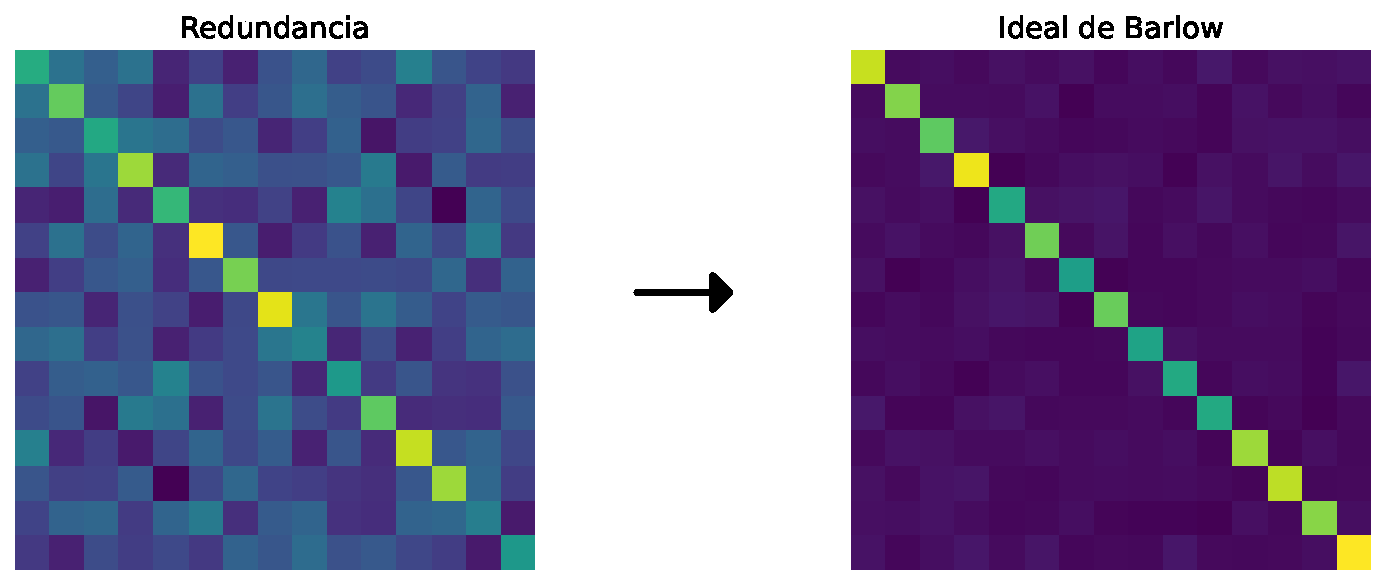
\includegraphics[width=0.9\textwidth]{heatmaps_IZ.pdf}
    \caption{Visualización conceptual de la matriz de información mutua $\mathcal{I}(Z)$ (simétrica), donde los ejes representan las neuronas de la capa de salida, o equivalentemente, las dimensiones de la codificación. La primera matriz corresponde a una representación redundante, donde existen dependencias significativas entre distintas componentes (valores no despreciables fuera de la diagonal). En el \textit{Ideal de Barlow}, la matriz presenta una estructura casi diagonal, donde las componentes son mutuamente independientes y cada una retiene su entropía individual máxima.}
    \label{fig:heatmaps_IZ}
\end{figure}

\subsection{El Puente de Jaynes}

Estimar la información mutua y la entropía de Shannon es computacionalmente intratable en espacios no triviales donde se desconoce la distribución subyacente de los datos. Sin embargo, cuando los datos se distribuyen de forma gaussiana, la expresión de la información mutua se reduce a una expresión que depende exclusivamente del coeficiente de correlación lineal de Pearson ($\rho_{ij}$).

\begin{proposition}[Puente de Jaynes]
Sea $(z_i, z_j)$ un par de representaciones distribuidas conjuntamente según una distribución normal con coeficiente de correlación de Pearson $\rho_{ij}$. Entonces, la información mutua de Shannon entre ambas variables viene dada por:
\begin{equation}
I(z_i; z_j) = -\frac{1}{2} \log(1 - \rho_{ij}^2)
\end{equation}
\end{proposition}

\begin{proof}
Sea $(z_i, z_j)$ siguiendo una distribución normal bivariante:
\begin{equation}
\begin{pmatrix} z_i \\ z_j \end{pmatrix} \sim \mathcal{N}\left( \begin{pmatrix} \mu_i \\ \mu_j \end{pmatrix}, \Sigma \right)
\end{equation}
Recordemos la funcion de densidad normal multivariante en el caso general:
\begin{equation}
p(Z) = \frac{1}{\sqrt{(2\pi)^k det(\Sigma)}} e^{ -\frac{1}{2}(Z-\mu)^\top \Sigma^{-1} (Z-\mu) }
\end{equation}

Aplicando la definición de entropía de Shannon y las propiedades del logaritmo:
\begin{equation}
\begin{aligned}
H(Z) &= \mathbb{E}[-\log p(Z)] \\
     &= \mathbb{E}\left[ \frac{1}{2} \log((2\pi)^k det(\Sigma)) + \frac{1}{2}(Z-\mu)^\top \Sigma^{-1} (Z-\mu) \right] \\
     &= \frac{1}{2} \log((2\pi)^k det(\Sigma)) + \frac{1}{2}\mathbb{E}\left[(Z-\mu)^\top \Sigma^{-1} (Z-\mu) \right]
\end{aligned}
\end{equation}

Aplicando $A \in \mathbb{R} \implies Tr(A) = A $ , $Tr(AB) = Tr(BA)$, $\Sigma = \mathbb{E}[(Z-\mu)(Z-\mu)^\top$:

\begin{equation}
\begin{aligned}
 \mathbb{E}\left[(Z-\mu)^\top \Sigma^{-1} (Z-\mu) \right] &= \mathbb{E}[\text{tr}((Z-\mu)^\top\Sigma^{-1} (Z-\mu))] \\ &= \text{tr}(\Sigma^{-1} \mathbb{E}[(Z-\mu)(Z-\mu)^\top]) \\ 
 &= \text{tr}(\Sigma^{-1} \Sigma) = \text{tr}(I_k) \\ 
 &= k
\end{aligned}
\end{equation}

Sustituyendo, agrupando y usando las propiedades de los logaritmos:
\begin{equation}
\begin{aligned}
H(Z) &= \frac{1}{2} \log((2\pi)^2 det(\Sigma)) + \frac{k}{2} \\ 
     &= \frac{1}{2} \log((2\pi)^2 det(\Sigma)) + \frac{1}{2}\log(e^k) \\
     &= \frac{1}{2} \log \left( (2\pi e)^k det(\Sigma) \right)
\end{aligned}
\end{equation}

Para evaluar la entropía conjunta $H(z_i, z_j)$, aplicamos la fórmula anterior particularizada para el caso $k=2$. Usando la relación $\Sigma_{ij} = \rho_{ij}\sqrt{\Sigma_{ii}\Sigma_{jj}}$, calculamos el determinante de la matriz de covarianza:

\begin{equation}
\begin{aligned} 
det(\Sigma) &= \Sigma_{ii}\Sigma_{jj} - \Sigma_{ij}^2 \\
            &= \Sigma_{ii}\Sigma_{jj} - \left( \rho_{ij}\sqrt{\Sigma_{ii}\Sigma_{jj}} \right)^2 \\
            &= \Sigma_{ii}\Sigma_{jj} - \rho_{ij}^2 \Sigma_{ii}\Sigma_{jj} \\ 
            &= \Sigma_{ii}\Sigma_{jj}(1 - \rho_{ij}^2)
\end{aligned}
\end{equation}

Por tanto la expresión de la entropía queda:
\begin{equation}
H(z_i, z_j) = \frac{1}{2} \log \left( (2\pi e)^2 \Sigma_{ii}\Sigma_{jj} (1 - \rho_{ij}^2) \right)
\end{equation}

Por su parte, las distribuciones marginales $p(z_i)$ y $p(z_j)$ resultan ser también gaussianas, pero en este caso unidimensionales ($k=1$), con varianzas $\Sigma_{ii}$ y $\Sigma_{jj}$ respectivamente. Por tanto, sus entropías marginales individuales son:
\begin{equation}
H(z_i) = \frac{1}{2} \log(2\pi e \Sigma_{ii}), \quad H(z_j) = \frac{1}{2} \log(2\pi e \Sigma_{jj})
\end{equation}

Aplicando la definición de información mutua y usando las propiedades algebraicas del logaritmo:
\begin{equation}
\begin{aligned}
I(z_i; z_j) &= H(z_i) + H(z_j) - H(z_i, z_j) \\
            &= \frac{1}{2} \log(2\pi e \Sigma_{ii}) + \frac{1}{2} \log(2\pi e \Sigma_{jj}) - \frac{1}{2} \log \left( (2\pi e)^2 \Sigma_{ii}\Sigma_{jj} (1 - \rho_{ij}^2) \right) \\
            &= \frac{1}{2} \log \left( \frac{(2\pi e \Sigma_{ii})(2\pi e \Sigma_{jj})}{(2\pi e)^2 \Sigma_{ii}\Sigma_{jj} (1 - \rho_{ij}^2)} \right) \\
            &= \frac{1}{2} \log \left( \frac{(2\pi e)^2 \Sigma_{ii}\Sigma_{jj}}{(2\pi e)^2 \Sigma_{ii}\Sigma_{jj} (1 - \rho_{ij}^2)} \right) \\
            &= -\frac{1}{2} \log(1 - \rho_{ij}^2)
\end{aligned}
\end{equation}
\end{proof}

En consecuencia, bajo el supuesto de que las representaciones siguen una distribución gaussiana, la correlación lineal basta para capturar la totalidad de las dependencias estadísticas. En este caso forzar la decorrelación lineal es suficiente para garantizar la independencia. El siguiente corolario muestra cómo esto nos permite simplificar la optimización de la matriz de información mutua $\mathcal{I}(Z)$:

\begin{corollary}[Equivalencia Matricial]
Sea $Z \in \mathbb{R}^d$ un vector de representaciones que sigue una distribución normal multivariante, $\mathcal{I}(Z) \in \mathbb{R}^{d \times d}$ su matriz de información mutua y $R \in \mathbb{R}^{d \times d}$ su matriz de correlación lineal. Bajo la hipótesis de normalidad, garantizar la independencia es equivalente a imponer la decorrelación lineal:
\begin{equation}
\mathcal{I}(Z) \text{ es diagonal } \iff R = I_d
\end{equation}
donde $I_d$ denota la matriz identidad de dimensión $d$.
\end{corollary}

\begin{proof}
Por definición, los elementos de la diagonal principal de cualquier matriz de correlación $R$ son iguales a la unidad ($R_{ii} = \rho_{ii} = 1$). Para los elementos fuera de la diagonal ($i \neq j$), la proposición del Puente de Jaynes establece que:
\begin{equation}
I(z_i; z_j) = -\frac{1}{2} \log(1 - \rho_{ij}^2)
\end{equation}

La matriz $\mathcal{I}(Z)$ es diagonal si y solo si la información mutua entre características distintas es nula, es decir, $I(z_i; z_j) = 0$ para todo $i \neq j$. Igualando a cero la expresión matricial obtenemos:
\begin{equation}
-\frac{1}{2} \log(1 - \rho_{ij}^2) = 0 \iff \log(1 - \rho_{ij}^2) = 0 \iff 1 - \rho_{ij}^2 = 1 \iff \rho_{ij} = 0
\end{equation}

Por consiguiente, exigir que $I(z_i; z_j) = 0$ para todo $i \neq j$ equivale a imponer que $\rho_{ij} = 0$ para todo $i \neq j$. Dado que los elementos diagonales de $R$ son iguales a $1$, esta condición equivale a $R = I_d$.
\end{proof}

\section{La Arquitectura Barlow Twins}
\label{sec:barlow_twins}

Propuesto por Zbontar et al. en 2021 \cite{zbontar2021barlow}, el método Barlow Twins traduce el principio de reducción de redundancia de Barlow de la sección anterior a un marco práctico de aprendizaje auto-supervisado.

\begin{figure}[H]
    \centering
    \begin{tikzpicture}[
        node distance=1.5cm and 2cm,
        box/.style={draw, rectangle, rounded corners, minimum width=2.2cm, minimum height=1.2cm, align=center, fill=blue!5},
        img/.style={draw, rectangle, rounded corners, minimum width=1.5cm, minimum height=1.5cm, fill=orange!10, align=center},
        mat/.style={draw, rectangle, minimum width=2.5cm, minimum height=2.5cm, fill=green!5, align=center},
        arrow/.style={->, >=stealth, thick}
    ]
        \node (x) {Observación $x$};
        \node[img, above right=0.5cm and 0.8cm of x] (ya) {Vista $A$\\$x_1 = t^A(x)$};
        \node[img, below right=0.5cm and 0.8cm of x] (yb) {Vista $B$\\$x_2 = t^B(x)$};
        \node[box, right=0.8cm of ya] (enc_a) {Red\\$f_\theta$};
        \node[box, right=0.8cm of yb] (enc_b) {Red\\$f_\theta$};
        \node[right=0.6cm of enc_a] (za) {$z^A$};
        \node[right=0.6cm of enc_b] (zb) {$z^B$};
        \node[mat, right=1.2cm of za, yshift=-1.6cm] (matrix) {Correlación\\Cruzada $C$};
        \node[right=0.8cm of matrix, font=\Large] (identidad) {$I_d$};
        
        \draw[arrow] (x.east) to[out=0, in=180] (ya.west);
        \draw[arrow] (x.east) to[out=0, in=180] (yb.west);
        \draw[arrow] (ya) -- (enc_a);
        \draw[arrow] (yb) -- (enc_b);
        \draw[arrow] (enc_a) -- (za);
        \draw[arrow] (enc_b) -- (zb);
        \draw[arrow] (za.east) to[out=0, in=180] (matrix.150);
        \draw[arrow] (zb.east) to[out=0, in=180] (matrix.210);
        \draw[<->, >=stealth, thick, red] (matrix.east) -- node[above, text=black] {$\mathcal{L}_{\mathcal{BT}}$} (identidad.west);
        \draw[<->, dashed, thick, gray] (enc_a.south) -- node[right, text=black, align=center, text width=2.5cm] {Pesos compartidos} (enc_b.north);
    \end{tikzpicture}
    \caption{Esquema de arquitectura Barlow Twins. Dos transformaciones aleatorias $t^A$ y $t^B$ generan vistas distorsionadas de $x$. Ambas se procesan con redes siamesas $f_\theta$ para obtener $z^A$ y $z^B$. Se calcula la matriz de correlación cruzada $C$ sobre el minibatch y se minimiza su discrepancia respecto a $I_d$.}
    \label{fig:barlow_twins_arch}
\end{figure}

\subsection{Construcción de las Vistas y Representaciones}

Dada una observación $x$, se generan dos vistas $x_1$ y $x_2$ mediante transformaciones aleatorias independientes $t^A, t^B$ (p.e. recortes, \textit{masking}, variaciones de color). Ambas vistas $x_1 = t^A(x)$ y $x_2 = t^B(x)$ se procesan con la misma red $f_\theta$ (pesos compartidos), produciendo dos representaciones vectoriales en $\mathbb{R}^d$:
\begin{equation}
z^A = f_\theta(x_1), \qquad z^B = f_\theta(x_2).
\end{equation}
En un escenario ideal donde el modelo fuese totalmente invariante a las transformaciones aplicadas, se cumpliría $z^A = z^B$. Sobre un minibatch de $N$ pares compatibles $\{(x_1^{(i)}, x_2^{(i)})\}_{i=1}^N$, apilamos las representaciones de cada vista en una matriz de batch:
\begin{equation}
Z^A, Z^B \in \mathbb{R}^{N \times d}, \qquad \text{donde la fila } i \text{ de } Z^A \text{ es } z^{A,(i)} = f_\theta(x_1^{(i)}) \in \mathbb{R}^d,
\end{equation}
y análogamente para $Z^B$ con $z^{B,(i)} = f_\theta(x_2^{(i)})$. Cada fila es una observación del minibatch; cada columna representa una dimensión del espacio latente. Denotaremos por $z_k^{A,(i)}$ la entrada $(i,k)$ de $Z^A$, es decir, el valor de la dimensión $k$ de la representación de la vista $A$ para la observación $i$.

\subsection{El Centrado en Media}

Antes de poder hablar de correlación, las representaciones deben estar \textbf{centradas en media}: para cada vista y cada dimensión $k$, se resta su media empírica sobre el minibatch,
\begin{equation}
z_k^{A,(i)} \gets z_k^{A,(i)} - \frac{1}{N}\sum_{m=1}^N z_k^{A,(m)}, \qquad z_k^{B,(i)} \gets z_k^{B,(i)} - \frac{1}{N}\sum_{m=1}^N z_k^{B,(m)},
\end{equation}
Esto centra cada columna de $Z^A$ y de $Z^B$ a media cero. La razón de exigir esto es simple: si las representaciones no estuvieran centradas, el producto escalar entre columnas estaría dominado por un término de medias de magnitud elevada, enmascarando la verdadera covarianza entre dimensiones. El centrado garantiza que lo que optimicemos a continuación sean auténticas correlaciones, y no simples momentos de segundo orden no centrados.

\subsection{La Matriz de Correlación Cruzada}

Con $Z^A, Z^B \in \mathbb{R}^{N \times d}$ (ya centradas por columnas), denotemos por $\mathbf{z}_k^A, \mathbf{z}_l^B \in \mathbb{R}^N$ la columna $k$-ésima de $Z^A$ y la columna $l$-ésima de $Z^B$, respectivamente, es decir, $\mathbf{z}_k^A = (z_k^{A,(1)}, \dots, z_k^{A,(N)})^\top$.

\begin{definition}[Matriz de Correlación Cruzada Empírica]
La matriz de correlación cruzada $C \in \mathbb{R}^{d \times d}$ se define entrada a entrada como la similitud coseno entre las columnas $k$-ésima de $Z^A$ y $l$-ésima de $Z^B$:
\begin{equation}
C_{kl} = \frac{\langle \mathbf{z}_k^A, \mathbf{z}_l^B \rangle}{\|\mathbf{z}_k^A\|_2 \, \|\mathbf{z}_l^B\|_2} = \frac{\sum_{i=1}^{N} z_k^{A,(i)} z_l^{B,(i)}}{\sqrt{\sum_{i=1}^{N} (z_k^{A,(i)})^2} \sqrt{\sum_{i=1}^{N} (z_l^{B,(i)})^2}}, \qquad C_{kl} \in [-1,1].
\end{equation}
Equivalentemente, en notación matricial: $C = (Z^A)^\top Z^B$ tras normalizar cada columna de $Z^A$ y $Z^B$ a norma unidad.
\end{definition}

\begin{figure}[H]
    \centering
    % El uso de \resizebox asegura que la figura nunca exceda el ancho de la página.
    % Requiere tener \usepackage{graphicx} en el preámbulo.
    \resizebox{\linewidth}{!}{
    \begin{tikzpicture}[
        every node/.style={font=\footnotesize},
        mathnode/.style={font=\footnotesize, minimum width=0.6cm, minimum height=0.45cm},
        highlight/.style={fill=orange!15, draw=orange!70!black, thick},
        highlightB/.style={fill=blue!10, draw=blue!60!black, thick},
        cellhighlight/.style={fill=green!15, draw=green!50!black, thick}
    ]

    % ============================================================
    % MATRIZ Z^A
    % ============================================================
    \matrix (ZA) [
        matrix of math nodes,
        nodes={mathnode},
        ampersand replacement=\&,
        left delimiter={(}, right delimiter={)},
        column sep=1pt, row sep=1pt,
        anchor=center
    ]
    {
        z_1^{A,(1)} \& \cdots \& z_k^{A,(1)} \& \cdots \& z_d^{A,(1)} \\
        z_1^{A,(2)} \& \cdots \& z_k^{A,(2)} \& \cdots \& z_d^{A,(2)} \\
        \vdots      \&        \& \vdots      \&        \& \vdots      \\
        z_1^{A,(N)} \& \cdots \& z_k^{A,(N)} \& \cdots \& z_d^{A,(N)} \\
    };
    \begin{scope}[on background layer]
        \node[highlight, fit=(ZA-1-3)(ZA-4-3), inner sep=1pt] (colA) {};
    \end{scope}
    \node[above=0.1cm of ZA] {$Z^A \in \mathbb{R}^{N \times d}$};
    \node[below=0.1cm of colA, text=orange!70!black] {dimensión $k$: $\mathbf{z}_k^A$};
    \node[font=\footnotesize, text=gray!80!black, rotate=90] at ([xshift=-0.6cm]ZA.west) {$\longleftarrow$ observaciones $\longrightarrow$};

    % ============================================================
    % MATRIZ Z^B
    % ============================================================
    \matrix (ZB) [
        matrix of math nodes,
        nodes={mathnode},
        ampersand replacement=\&,
        left delimiter={(}, right delimiter={)},
        column sep=1pt, row sep=1pt,
        anchor=center,
        right=0.6cm of ZA
    ]
    {
        z_1^{B,(1)} \& \cdots \& z_l^{B,(1)} \& \cdots \& z_d^{B,(1)} \\
        z_1^{B,(2)} \& \cdots \& z_l^{B,(2)} \& \cdots \& z_d^{B,(2)} \\
        \vdots      \&        \& \vdots      \&        \& \vdots      \\
        z_1^{B,(N)} \& \cdots \& z_l^{B,(N)} \& \cdots \& z_d^{B,(N)} \\
    };
    \begin{scope}[on background layer]
        \node[highlightB, fit=(ZB-1-3)(ZB-4-3), inner sep=1pt] (colB) {};
    \end{scope}
    \node[above=0.1cm of ZB] {$Z^B \in \mathbb{R}^{N \times d}$};
    \node[below=0.1cm of colB, text=blue!60!black] {dimensión $l$: $\mathbf{z}_l^B$};

    % ============================================================
    % MATRIZ C
    % ============================================================
    \matrix (C) [
        matrix of math nodes,
        nodes={mathnode},
        ampersand replacement=\&,
        left delimiter={(}, right delimiter={)},
        column sep=1pt, row sep=1pt,
        anchor=center,
        right=0.6cm of ZB
    ]
    {
        C_{11} \& \cdots \& C_{1l} \& \cdots \& C_{1d} \\
        \vdots \&        \& \vdots \&        \& \vdots \\
        C_{k1} \& \cdots \& C_{kl} \& \cdots \& C_{kd} \\
        \vdots \&        \& \vdots \&        \& \vdots \\
        C_{d1} \& \cdots \& C_{dl} \& \cdots \& C_{dd} \\
    };
    \begin{scope}[on background layer]
        \node[cellhighlight, fit=(C-3-3), inner sep=1pt] (cellKL) {};
    \end{scope}
    \node[above=0.1cm of C] {$C \in \mathbb{R}^{d \times d}$};

    % ============================================================
    % FÓRMULA CENTRAL
    % ============================================================
    \node[
        below=0.6cm of C,
        anchor=center
    ] (dotprod) {
        \textcolor{green!50!black}{$C_{kl}$} $= \dfrac{\langle {\mathbf{z}_k^A}, {\mathbf{z}_l^B} \rangle}
        {\|{\mathbf{z}_k^A}\|_2 \, \|{\mathbf{z}_l^B}\|_2}$
    };

    \end{tikzpicture}
    }
    \caption{Construcción de la matriz de correlación cruzada $C$ mediante el producto escalar normalizado (similitud coseno) entre las columnas de $Z^A$ y $Z^B$.}
    \label{fig:cross_corr_matrices_horizontal_compact}
\end{figure}

\begin{definition}[Función de Pérdida de Barlow Twins]
La pérdida penaliza la discrepancia de $C$ respecto a la identidad $I_d$:
\begin{equation}
\mathcal{L}_{\mathcal{BT}} = \underbrace{\sum_{k=1}^{d} (1 - C_{kk})^2}_{\text{Invarianza}} + \lambda \underbrace{\sum_{k=1}^{d} \sum_{l \neq k} C_{kl}^2}_{\text{Redundancia}},
\end{equation}
\end{definition} 
\noindent siendo $\lambda > 0$ un hiperparámetro que pondera los dos objetivos de la pérdida. Análogamente a cómo el margen en las pérdidas contrastivas regula la repulsión entre muestras negativas, aquí $\lambda$ modula la repulsión \textit{entre características}. Cada término de $\mathcal{L}_{\mathcal{BT}}$ tiene una interpretación geométrica derivada de la construcción de $C$:

\begin{itemize}
    \item \textbf{Invarianza ($C_{kk} \to 1$):} $C_{kk}$ es la similitud coseno entre la columna $k$ de $Z^A$ y la columna $k$ de $Z^B$, es decir, entre los valores que la dimensión $k$ asume en la vista $A$ y en la vista $B$ a lo largo de todo el minilote. Forzar $C_{kk} \to 1$ exige que ambas columnas sean proporcionales en $\mathbb{R}^N$; por la desigualdad de Cauchy-Schwarz, esto ocurre si y solo si $\mathbf{z}_k^A = c \cdot \mathbf{z}_k^B$ con $c > 0$, es decir, que la red extraiga la misma información en la dimensión $k$ con independencia de la vista procesada.

    \item \textbf{Reducción de redundancia ($C_{kl} \to 0$, $k \neq l$):} durante el entrenamiento las vistas difieren ($Z^A \neq Z^B$), por lo que $C_{kl}$ captura la correlación cruzada entre la dimensión $k$ de la vista $A$ y la dimensión $l$ de la vista $B$. Forzar $C_{kl} \to 0$ equivale a imponer $\langle \mathbf{z}_k^A, \mathbf{z}_l^B \rangle \to 0$, es decir, ortogonalidad cruzada entre dimensiones distintas de las dos vistas. Cada dimensión queda así obligada a codificar información que las demás no capturan, repartiendo la varianza semántica por todo $\mathbb{R}^d$ de acuerdo con el principio de Barlow.
\end{itemize}

La matriz empírica $C$ aproxima, en cada minibatch, la correlación cruzada poblacional $\mathcal{C}_{kl} = \mathbb{E}[Z_k^A Z_l^B] / \sqrt{\mathbb{E}[(Z_k^A)^2]\mathbb{E}[(Z_l^B)^2]}$ definida sobre la distribución de pares positivos $p_{\text{pos}}(x_1,x_2)$. Barlow Twins emplea la correlación \textit{cruzada} en lugar de la autocorrelación precisamente porque, durante el entrenamiento, $Z^A \neq Z^B$: al operar con $C$, el método mide y minimiza simultáneamente la discrepancia entre vistas en la diagonal y la redundancia entre características fuera de ella.

La conexión con la teoría de Barlow se vuelve exacta en el \textbf{límite de invarianza perfecta}. Cuando el modelo asimila ambas vistas idénticamente ($Z^A = Z^B = Z$), cada par de columnas colapsa a un único vector ($\mathbf{z}_k^A = \mathbf{z}_k^B = \mathbf{z}_k$), y la correlación cruzada $\mathcal{C}$ se reduce a la matriz de autocorrelación de Pearson $R$ de la Sección~\ref{sec:barlow_hipotesis}. En ese límite, forzar $\mathcal{C} \to I_d$ equivale estrictamente a imponer $R \to I_d$, logrando la decorrelación que exige el principio original.


En resumen, Barlow Twins evita el colapso de las \textit{Joint Embedding Architectures} sin recurrir a muestras negativas ni a mecanismos arquitectónicos auxiliares. Basta con imponer $C \to I_d$, condición que, como establece el Puente de Jaynes (Sección~\ref{sec:barlow_hipotesis}), es matemáticamente equivalente a exigir la independencia estadística entre las dimensiones del espacio $\mathcal{Z}$.

\section{VICReg: Desacoplamiento de Varianza, Invarianza y Covarianza}
\label{sec:vicreg}

La elección de la matriz de correlación cruzada $C$ como objeto central de la optimización en Barlow Twins conlleva algunos problemas de diseño. Recordemos que cada entrada $C_{kl}$ se obtiene dividiendo el producto escalar entre las columnas $\mathbf{z}_k^A$ y $\mathbf{z}_l^B$ por el producto de sus normas euclídeas. Esto hace que el objeto de optimización ignore la escala de las representaciones, centrándose únicamente en las direcciones.

\begin{proposition}[Invarianza de $C$ ante reescalado]
\label{prop:C_escala}
Sea $C$ la matriz de correlación cruzada definida en la Sección~\ref{sec:barlow_twins}. Para cualquier reescalado positivo por dimensiones $z_j \mapsto \alpha_j z_j$ con $\alpha_j > 0$, la matriz $C$ permanece inalterada.
\end{proposition}

\begin{proof}
Sea $\tilde{\mathbf{z}}_k^A = \alpha_k \mathbf{z}_k^A$ la columna $k$-ésima de $Z^A$ tras el reescalado. Entonces:
\begin{equation}
\tilde{C}_{kl} = \frac{\langle \tilde{\mathbf{z}}_k^A, \tilde{\mathbf{z}}_l^B \rangle}{\|\tilde{\mathbf{z}}_k^A\|_2 \, \|\tilde{\mathbf{z}}_l^B\|_2} = \frac{\alpha_k \alpha_l \langle \mathbf{z}_k^A, \mathbf{z}_l^B \rangle}{\alpha_k \|\mathbf{z}_k^A\|_2 \cdot \alpha_l \|\mathbf{z}_l^B\|_2} = \frac{\langle \mathbf{z}_k^A, \mathbf{z}_l^B \rangle}{\|\mathbf{z}_k^A\|_2 \, \|\mathbf{z}_l^B\|_2} = C_{kl}.
\end{equation}
Los factores $\alpha_k$ y $\alpha_l$ se cancelan exactamente por la normalización.
\end{proof}

Por tanto, la formulación Barlow Twins basada en la matriz de correlación cruzada $C$ presenta dos problemas fundamentales que limitan su capacidad de regularización:

\begin{enumerate}
    \item Colapso dimensional por ausencia de sensibilidad a la escala.
    \item Acoplamiento de objetivos (\textit{entanglement}).
\end{enumerate}

Respecto al primer problema, la Proposición~\ref{prop:C_escala} implica que $C$ descarta toda información sobre la \emph{escala} de las dimensiones de $\mathcal{Z}$. En particular, reducir la varianza de una dimensión $j$ a un valor arbitrariamente pequeño no modifica los elementos diagonales $C_{jj}$ ya que están normalizados. Recordemos que si una dimensión tiene varianza nula, significa que la red está emitiendo exactamente el mismo valor numérico para todas las imágenes a lo largo de esa coordenada; esta es precisamente la manifestación empírica del colapso dimensional. Esto plantea un grave problema, una dimensión colapsada (cuya varianza tiende a cero por no codificar información útil) puede mantener un valor óptimo $C_{jj} \approx 1$ siempre que las fluctuaciones residuales en $\mathbf{z}_j^A$ y $\mathbf{z}_j^B$ estén alineadas. La pérdida $\mathcal{L}_{\mathcal{BT}}$ no distingue entre una dimensión con varianza unitaria y otra con varianza despreciable, ambas contribuyen de forma idéntica a la diagonal de $C$. Por tanto, $\mathcal{L}_{\mathcal{BT}}$ carece de un mecanismo explícito para garantizar que todas las dimensiones del espacio $\mathcal{Z}$ mantengan una dispersión suficiente.

El segundo problema surge de condensar los objetivos de invarianza ($C_{kk} \to 1$) y de decorrelación ($C_{kl} \to 0$) en un único objeto, la matriz $C$. Como ambos términos comparten el mismo denominador de normalización, no pueden tratarse de forma independiente: cualquier perturbación se propaga simultáneamente a la diagonal y a la parte fuera de la diagonal de $C$, acoplando así dos objetivos que, en principio, son conceptualmente distintos, Bardes et al.~\cite{bardes2022vicreg}.

Resulta natural preguntarse si es posible evitar estas limitaciones formulando una función de pérdida que \emph{desacople} explícitamente la invarianza, la dispersión dimensional y la independencia entre características, sobre un objeto que retenga la información de escala que $C$ descarta. VICReg (\textit{Variance-Invariance-Covariance Regularization}), propuesto por Bardes, Ponce y LeCun en 2022~\cite{bardes2022vicreg}, ofrece dicha formulación.

\subsection{De la correlación cruzada a la covarianza}

\begin{definition}[Matriz de Covarianza Empírica]
\label{def:cov_empirica_vicreg}
Sea $Z \in \mathbb{R}^{N \times d}$ una matriz de embeddings correspondiente a un batch de $N$ observaciones, y sea $\bar{z} = \frac{1}{N}\sum_{i=1}^{N} z^{(i)} \in \mathbb{R}^d$ su vector de medias. La matriz de covarianza empírica se define como:
\begin{equation}
\label{eq:cov_empirica_vicreg}
\Sigma_\mathcal{Z} = \frac{1}{N-1} \sum_{i=1}^{N} (z^{(i)} - \bar{z})(z^{(i)} - \bar{z})^\top = \frac{1}{N-1} (Z - \bar{Z})^\top (Z - \bar{Z}) \in \mathbb{R}^{d \times d},
\end{equation}
donde $\bar{Z} \in \mathbb{R}^{N \times d}$ denota la matriz cuyas $N$ filas son todas iguales a $\bar{z}^\top$. El elemento $(\Sigma_\mathcal{Z})_{kl}=\operatorname{Cov}(z_{k},z_{l})$ es la covarianza empírica entre las dimensiones $k$ y $l$ a lo largo del batch, y en particular $(\Sigma_\mathcal{Z})_{jj} = \operatorname{Var}(z_{j})$ es la varianza empírica de la dimensión $j$.
\end{definition}

La idea central de VICReg consiste en usar esta matriz de covarianza empírica en lugar de la matriz de correlación cruzada $C$ de la Sección~\ref{sec:barlow_twins}. Nótese que este objeto ya fue introducido en un contexto poblacional en la Sección~\ref{sec:colapso_dimensional_v2}; aquí empleamos su versión empírica, o estimador sobre el batch. A diferencia de $C$, cuyos elementos satisfacen $C_{kl} \in [-1,1]$ por construcción, los elementos de $\Sigma_\mathcal{Z}$ no están acotados ni normalizados. Para comprender qué información pierde $C$ respecto a $\Sigma_\mathcal{Z}$, veremos la relación entre ambos objetos.

En el límite analizado al final de la Sección~\ref{sec:barlow_twins} ($Z^A = Z^B = Z$), la correlación cruzada $C$ se reduce a la matriz de autocorrelación $R$ de una única vista. La relación entre $R$ y la covarianza $\Sigma_\mathcal{Z}$ de un mismo vector aleatorio es la siguiente: 
\begin{equation}
\label{eq:relacion_R_Sigma}
R_{kl} = \frac{(\Sigma_\mathcal{Z})_{kl}}{\sqrt{(\Sigma_\mathcal{Z})_{kk}}\,\sqrt{(\Sigma_\mathcal{Z})_{ll}}}.
\end{equation}

La ecuación~\eqref{eq:relacion_R_Sigma} muestra que $R$ y por extensión $C$ en el límite de invarianza (i.e. cuando la red aprende $Z^A = Z^B = Z$) pueden reconstruirse a partir de $\Sigma_\mathcal{Z}$. Sin embargo, la operación inversa no es posible: dada $R$, no se pueden recuperar las varianzas que la normalización ha eliminado. Observando la estructura de ambas matrices:
\begin{equation*}
C = 
\begin{pmatrix}
1 & C_{12} & \cdots & C_{1d} \\
C_{21} & 1 & \cdots & C_{2d} \\
\vdots & \vdots & \ddots & \vdots \\
C_{d1} & C_{d2} & \cdots & 1
\end{pmatrix}
\quad  \quad
\Sigma_\mathcal{Z} = 
\begin{pmatrix}
\sigma_1^2 & \Sigma_{12} & \cdots & \Sigma_{1d} \\
\Sigma_{21} & \sigma_2^2 & \cdots & \Sigma_{2d} \\
\vdots & \vdots & \ddots & \vdots \\
\Sigma_{d1} & \Sigma_{d2} & \cdots & \sigma_d^2
\end{pmatrix}
\end{equation*}
La diagonal de $\Sigma_\mathcal{Z}$ retiene explícitamente las varianzas individuales $\sigma_j^2 = (\Sigma_\mathcal{Z})_{jj}$, mientras que la diagonal de $C$ es idénticamente 1 por construcción. En conclusión, $\Sigma_\mathcal{Z}$ contiene estrictamente más información que $R$.


Operar sobre $\Sigma_\mathcal{Z}$ en lugar de sobre $C$ permite descomponer el problema de optimización en tres objetivos independientes: varianza, invarianza y covarianza. Cada uno de estos términos resuelve una de las limitaciones de Barlow Twins identificadas anteriormente. El término de varianza opera directamente sobre la diagonal de $\Sigma_\mathcal{Z}$, preservando así la información sobre la dispersión de cada dimensión y resolviendo el problema de la escala. El término de covarianza opera, a su vez, sobre la parte fuera de la diagonal de $\Sigma_\mathcal{Z}$, heredando así el papel de decorrelación que antes desempeñaba $C$. El término de invarianza (optimizar para que $z^A \approx z^B$), por su parte, se extrae fuera de la matriz y se mide mediante una función independiente que actúa directamente sobre las representaciones, resolviendo así el problema del acoplamiento. Formalizamos a continuación cada uno de estos tres términos.
\subsection{Término de Invarianza}

Como se introdujo en el Capítulo~\ref{cap:siamesas_colapso}, el primer objetivo de cualquier \textit{Joint Embedding Architechture} es la invarianza, es decir, la red debe aprender que representaciones de dos vistas de una misma observación deben ser próximas ($z^A \approx z^B$). En Barlow Twins, este objetivo se codificaba indirectamente a través de la diagonal de $C$ ($C_{kk} \to 1$). Esta condición medía la similitud de las direcciones entre las columnas de $Z^A$ y $Z^B$, sin embargo "olvidaba" la magnitud. Para solucionar este problema, VICReg recupera la pérdida $\mathcal{L}_{\text{pos}}$ definida en el Capítulo~\ref{cap:siamesas_colapso}.

\begin{definition}[Término de Invarianza de VICReg]
\label{def:vicreg_invarianza}
Dados dos batches de embeddings $Z^A, Z^B \in \mathbb{R}^{N \times d}$ generados a partir de pares positivos $\{(x_1^{(i)}, x_2^{(i)})\}_{i=1}^N$, el término de invarianza se define como el error cuadrático medio entre las representaciones de cada par:
\begin{equation}
\label{eq:vicreg_inv}
\mathcal{L}_{\text{pos}}(Z^A, Z^B) = \frac{1}{N} \sum_{i=1}^{N} \| z^{A,(i)} - z^{B,(i)} \|_2^2.
\end{equation}
\end{definition}

Frente a la condición $C_{kk} \to 1$ de la Sección~\ref{sec:barlow_twins}, que opera sobre similitudes coseno agregadas a lo largo de todo el lote, la invarianza de VICReg actúa directamente sobre las diferencias punto a punto. Al no normalizar, $\mathcal{L}_{\text{pos}}$ penaliza tanto la dirección como la magnitud de la discrepancia entre vistas.

\subsection{Término de Varianza}

El término de invarianza $\mathcal{L}_{\text{pos}}$ por sí solo es insuficiente para entrenar la red. Como vimos en la Sección~\ref{sec:demostracion_colapso}, si la función de pérdida se redujera únicamente a $\mathcal{L}_{\text{pos}}(Z^A, Z^B)$, la red podría minimizarla trivialmente proyectando todas las observaciones al mismo punto constante $z^{A,(i)} = z^{B,(i)} = c$.

En Barlow Twins, el colapso se previene de forma implícita, forzando la ortogonalidad entre dimensiones mediante la penalización $C_{kl} \to 0$ para $k \neq l$, lo que indirectamente genera dispersión. Sin embargo, como muestra la Proposición~\ref{prop:C_escala}, la normalización de $C$ hace invisible cualquier reducción de varianza en dimensiones individuales. Si la red proyecta todas las observaciones a un mismo valor constante en la dimensión $j$, la dispersión de esa coordenada desaparece $\operatorname{Var}(z_j) \to 0$. Al no tener sensibilidad a la escala, $\mathcal{L}_{\mathcal{BT}}$ es incapaz de detectar que dicha dimensión ha colapsado y ha dejado de ser informativa.

VICReg resuelve este punto ciego introduciendo un término de regularización que actúa directamente sobre la información que la normalización de $C$ descartaba: la diagonal de la matriz de covarianza $\Sigma_\mathcal{Z}$, es decir, las varianzas individuales $\{(\Sigma_\mathcal{Z})_{jj}\}_{j=1}^d$ de cada dimensión del espacio latente.

\begin{definition}[Término de Varianza de VICReg]
\label{def:vicreg_varianza}
Sea $Z \in \mathbb{R}^{N \times d}$ un batch de embeddings y sea $\sigma_j(Z) = \sqrt{(\Sigma_\mathcal{Z})_{jj}}$, donde $(\Sigma_\mathcal{Z})_{jj}$ es la varianza empírica de la dimensión $j$. El término de varianza en la pérdida VICReg se define agregando estos valores a lo lardo de todas las dimensiones de $\mathcal{Z}$ cuando la dispersión es insuficiente:
\begin{equation}
\label{eq:vicreg_var}
\mathcal{L}_{\text{var}}(Z) = \frac{1}{d} \sum_{j=1}^{d} \max\left(0, \; 1 - \sigma_j(Z)\right).
\end{equation}
\end{definition}

\noindent La función \textit{máx} fija un umbral $\gamma = 1$ sobre la desviación estándar de cada dimensión:
\begin{itemize}
    \item Si $\sigma_j(Z) < 1$, la dimensión $j$ tiene una dispersión insuficiente en el batch y el término se activa: $\max(0, 1 - \sigma_j) = 1 - \sigma_j > 0$. La derivada $\partial \mathcal{L}_{\text{var}} / \partial \sigma_j = -1/d$ inyecta un gradiente que expande las representaciones a lo largo de esa dimensión, contrarrestando la fuerza contractiva de $\mathcal{L}_{\text{pos}}$.
    \item Si $\sigma_j(Z) \geq 1$, la dimensión ya posee dispersión suficiente y se desactiva: $\max(0, 1 - \sigma_j) = 0$. El término deja de intervenir, permitiendo que las demás componentes de la pérdida operen sin interferencia.
\end{itemize}

\subsection{Término de Covarianza}

El tercer objetivo es la reducción de redundancia. Siguiendo la Hipótesis de Barlow \cite{barlow1961possible}, las dimensiones del espacio latente deben codificar información independiente. En Barlow Twins, este objetivo se implementaba penalizando los elementos no diagonales de $C$ ($C_{kl} \to 0$, $k \neq l$). VICReg persigue el mismo fin, pero operando sobre la covarianza no normalizada.

\begin{definition}[Término de Covarianza de VICReg]
\label{def:vicreg_covarianza}
Sea $\Sigma_\mathcal{Z} \in \mathbb{R}^{d \times d}$ la matriz de covarianza empírica del lote, definida en~\eqref{eq:cov_empirica_vicreg}. El término de covarianza en la pérdida VICReg agrega los valores no diagonales:
\begin{equation}
\label{eq:vicreg_cov}
\mathcal{L}_{\text{cov}}(Z) = \frac{1}{d} \sum_{\substack{k,l=1 \\ k \neq l}}^{d} (\Sigma_\mathcal{Z})_{kl}^2.
\end{equation}
\end{definition}

Minimizar $\mathcal{L}_{\text{cov}}(Z)$ fuerza la decorrelación entre las dimensiones de $\mathcal{Z}$. La diferencia con el término de redundancia de Barlow Twins es que aquí se penaliza la covarianza absoluta $(\Sigma_\mathcal{Z})_{kl}$, no la correlación normalizada $C_{kl}$. Dos dimensiones con varianzas elevadas y covarianza moderada recibirán en VICReg una penalización proporcional a la magnitud absoluta de su dependencia lineal, mientras que en Barlow Twins la normalización podría atenuar esta señal.

\begin{remark}
\label{rem:vicreg_jaynes}
Como se introdujo al principio del capítulo, El Puente de Jaynes establece que, bajo la hipótesis de normalidad, la información mutua entre dos dimensiones depende exclusivamente del coeficiente de correlación de Pearson: $I(z_k; z_l) = -\frac{1}{2}\log(1 - \rho_{kl}^2)$. Dado que el coeficiente de correlación se expresa como:
\begin{equation}
\rho_{kl} = \frac{(\Sigma_\mathcal{Z})_{kl}}{\sqrt{(\Sigma_\mathcal{Z})_{kk}(\Sigma_\mathcal{Z})_{ll}}}
\end{equation}
 se tiene que $\rho_{kl} = 0$ si y solo si $(\Sigma_\mathcal{Z})_{kl} = 0$. Por tanto, forzar $(\Sigma_\mathcal{Z})_{kl} \to 0$ mediante el término $\mathcal{L}_{\text{cov}}(Z)$ es equivalente a forzar $\rho_{kl} \to 0$, lo que por el Puente de Jaynes garantiza $I(z_k; z_l) \to 0$. En otras palabras, bajo la hipótesis de normalidad, el término de covarianza de VICReg logra la misma independencia estadística que el término de redundancia de Barlow Twins, pero por una vía algebraicamente diferente: operando sobre covarianzas absolutas en lugar de correlaciones normalizadas.
\end{remark}

\subsection{La Función de Pérdida de VICReg}

Los tres términos definidos anteriormente operan sobre aspectos ortogonales de la geometría del espacio latente: la invarianza mide la proximidad \textit{entre} vistas, la varianza controla la dispersión \textit{dentro} de cada vista, y la covarianza regula la independencia \textit{entre dimensiones} de cada vista. La pérdida total se define de forma compacta mediante el producto escalar entre el vector de ponderaciones $\boldsymbol{\mu}$ y el vector de pérdidas individuales $\mathbf{L}(Z^A, Z^B)$:

\begin{definition}[Función de Pérdida de VICReg]
\label{def:vicreg_loss}
\begin{flalign*}
& \begin{aligned}[b]
\mathcal{L}_{\text{VICReg}} &= \langle \boldsymbol{\mu}, \mathbf{L}(Z^A, Z^B) \rangle \\
&= \mu_1 \mathcal{L}_{\text{pos}}(Z^A, Z^B) + \mu_2 \left[ \mathcal{L}_{\text{var}}(Z^A) + \mathcal{L}_{\text{var}}(Z^B) \right] + \mu_3 \left[ \mathcal{L}_{\text{cov}}(Z^A) + \mathcal{L}_{\text{cov}}(Z^B) \right]
\end{aligned} &
\end{flalign*}


donde el vector de hiperparámetros $\boldsymbol{\mu}$ y el vector de objetivos $\mathbf{L}(Z^A, Z^B)$ quedan definidos por:
\begin{equation}
\label{eq:vicreg_vectors}
\boldsymbol{\mu} = \begin{pmatrix} \mu_1 \\ \mu_2 \\ \mu_3 \end{pmatrix}, \quad 
\mathbf{L}(Z^A, Z^B) = \begin{pmatrix} \mathcal{L}_{\text{pos}}(Z^A, Z^B) \\ \mathcal{L}_{\text{var}}(Z^A) + \mathcal{L}_{\text{var}}(Z^B) \\ \mathcal{L}_{\text{cov}}(Z^A) + \mathcal{L}_{\text{cov}}(Z^B) \end{pmatrix}
\end{equation}
con $\mu_1, \mu_2, \mu_3 > 0$ indicando el peso de cada componente de la pérdida.
\end{definition}

Los términos de varianza y covarianza se aplican a $Z^A$ y $Z^B$ de forma independiente, regularizando propiedades geométricas internas de cada rama, mientras que la invarianza opera necesariamente sobre la relación entre ambas. Nótese el contraste con $\mathcal{L}_{\mathcal{BT}}$ (Sección~\ref{sec:barlow_twins}), con un único hiperparámetro $\lambda$ para modular el balance entre dos objetivos acoplados a través de $C$. En VICReg, los tres coeficientes son genuinamente independientes: ajustar $\mu_2$ no altera la contribución de $\mu_3$ ni de $\mu_1$, simplificando la calibración del método y reduce su sensibilidad al tamaño del batch~\cite{bardes2022vicreg}.

\begin{figure}[H]
\centering
\resizebox{\linewidth}{!}{
\begin{tikzpicture}[
    node distance=1cm,
    inputbox/.style={draw, rectangle, rounded corners, minimum width=1.8cm, minimum height=0.7cm, align=center, fill=gray!5, font=\footnotesize},
    matbox/.style={draw, rectangle, rounded corners, minimum width=2.5cm, minimum height=1cm, align=center, fill=green!5, font=\footnotesize},
    termbox/.style={draw, rectangle, rounded corners, minimum width=1.8cm, minimum height=0.9cm, align=center, font=\footnotesize},
    arrow/.style={->, >=stealth, thick}
]

% ===== BARLOW TWINS =====
\node[font=\small\bfseries\sffamily] (bt_title) at (0, 0) {$\mathcal{L}_{BT}$};

\node[inputbox] (bt_input) at (0, -1.2) {$Z^A, Z^B$};

\node[matbox] (bt_C) at (0, -3) {Correlaci\'on cruzada $C$\\{\scriptsize normalizada: $C_{kl} \in [-1,1]$}};

\node[termbox, fill=orange!12] (bt_inv) at (-1.8, -5) {$C_{kk} \to 1$\\{\scriptsize Invarianza}};
\node[termbox, fill=blue!10] (bt_red) at (1.8, -5) {$C_{kl} \to 0$\\{\scriptsize Redundancia}};

\draw[arrow] (bt_input) -- (bt_C);
\draw[arrow] (bt_C) to[out=-150, in=90] (bt_inv);
\draw[arrow] (bt_C) to[out=-30, in=90] (bt_red);

% Coupled grouping
\begin{scope}[on background layer]
    \node[draw=gray, dashed, rounded corners, fit=(bt_inv)(bt_red), inner sep=8pt, fill=gray!3] {};
\end{scope}


% ===== SEPARATOR =====
\draw[dashed, gray!50, thick] (3.75, 0.5) -- (3.75, -7.5);

% ===== VICREG =====
\node[font=\small\bfseries\sffamily] (vic_title) at (9, 0) {$\mathcal{L}_{\text{VICReg}}$};

\node[inputbox] (vic_input) at (9, -1.2) {$Z^A, Z^B$};

% Matriz de Covarianza Intermedia
\node[matbox] (vic_sigma) at (10.5, -3) {Covarianza $\Sigma_\mathcal{Z}$\\{\scriptsize $\Sigma_{Z^A}, \Sigma_{Z^B}$}};

% Losses
\node[termbox, fill=orange!12] (vic_s) at (6, -5) {$\mathcal{L}_{\text{pos}}(Z^A, Z^B)$\\{\scriptsize Invarianza}};
\node[termbox, fill=red!10] (vic_v) at (9, -5) {$\mathcal{L}_{\text{var}}(Z)$\\{\scriptsize Varianza}};
\node[termbox, fill=blue!10] (vic_c) at (12, -5) {$\mathcal{L}_{\text{cov}}(Z)$\\{\scriptsize Covarianza}};

% Flechas desde el Input
\draw[arrow] (vic_input.south) to[out=-150, in=90] (vic_s.north);
\draw[arrow] (vic_input.south) to[out=-30, in=90] (vic_sigma.north);

% Flechas desde la Matriz de Covarianza
\draw[arrow] (vic_sigma.south) to[out=-150, in=90] (vic_v.north);
\draw[arrow] (vic_sigma.south) to[out=-30, in=90] (vic_c.north);

% Independent grouping
\begin{scope}[on background layer]
    \node[draw=gray, dashed, rounded corners, fit=(vic_s)(vic_v)(vic_c), inner sep=10pt, fill=gray!3] {};
\end{scope}


\end{tikzpicture}
}
\caption{Comparativa estructural entre las funciones de p\'erdida de Barlow Twins y VICReg. \textbf{Izquierda:} Barlow Twins condensa invarianza y decorrelaci\'on en la matriz de correlaci\'on cruzada normalizada $C$, que por construcci\'on descarta la informaci\'on de escala (varianza). \textbf{Derecha:} VICReg desacopla los tres objetivos operando directamente sobre las representaciones (invarianza) y la matriz de covarianza no normalizada $\Sigma_\mathcal{Z}$ (varianza y covarianza), permitiendo un control independiente de cada aspecto geom\'etrico del espacio latente.}
\label{fig:bt_vs_vicreg}
\end{figure}

\section{Limitaciones}
\label{sec:conclusiones_barlow}

En este capítulo hemos desarrollado un argumento que parte de un principio neurobiológico desembocando en dos funciones de pérdida para el aprendizaje auto-supervisado.

\begin{enumerate}
    \item \textbf{El principio de Barlow}  postula que una representación eficiente es aquella cuyas componentes son estadísticamente independientes. El objetivo ideal es diagonalizar la matriz de información mutua $\mathcal{I}(Z)$.
    
    \item \textbf{El Puente de Jaynes} reduce este problema intratable a uno tratable. Bajo la hipótesis de normalidad, la independencia estadística equivale a la decorrelación lineal ($R = I_d$), permitiendo operar exclusivamente con momentos de segundo orden.
    
    \item \textbf{Barlow Twins y VICReg} materializan esta decorrelación mediante dos estrategias distintas: la primera opera sobre la correlación cruzada normalizada $C$; la segunda desacopla varianza, invarianza y covarianza operando directamente sobre $\Sigma_\mathcal{Z}$, resolviendo las limitaciones de escala y acoplamiento de la primera.
\end{enumerate}

\subsection{Dependencia de la Hipótesis Gaussiana}

Toda la teória presentada en este capítulo descansa sobre el Puente de Jaynes, que establece la equivalencia entre decorrelación lineal e independencia estadística \textit{únicamente} cuando las representaciones siguen una distribución normal multivariante. En la práctica, esta hipótesis no siempre se satisface. Las redes profundas pueden dar lugar a distribuciones complejas, multimodales o con dependencias no lineales que la correlación de Pearson no captura. En estos escenarios, dos dimensiones pueden tener correlación nula ($\rho_{kl} = 0$) y, sin embargo, compartir información mutua no nula $I(z_k; z_l) > 0$, invalidando la equivalencia del Puente de Jaynes.

Esta limitación implica que tanto Barlow Twins como VICReg, al operar exclusivamente sobre momentos de segundo orden, pueden declarar independencia entre dimensiones que en realidad mantienen dependencias de orden superior. El término de covarianza $\mathcal{L}_{\text{cov}}$ elimina las correlaciones lineales, pero no tiene acceso a las dependencias no lineales que la información mutua sí detectaría. En consecuencia, la reducción de redundancia lograda por estos métodos es, en el caso general, una \textit{aproximación} al ideal de Barlow, exacta solo bajo normalidad.

